\documentclass[../piano-di-progetto.tex]{subfiles}
\begin{document}
  \section{Preventivo}
  Di seguito verranno riportati i preventivi per le varie macro-fasi di lavoro. Sia la macro-fase di Analisi, sia la macro-fase di Consolidamento dei requisiti non verranno rendicontate nel preventivo finale in quanto vengono considerate come ore di investimento per l’approfondimento personale.

  Per facilitare la lettura delle seguenti tabelle, vengono utilizzate delle sigle per identificare i ruoli:
  \begin{itemize}
    \item \textbf{Re}: Responsabile;
    \item \textbf{Am}: Amministratore;
    \item \textbf{An}: Analista;
    \item \textbf{Pt}: Progettista;
    \item \textbf{Pr}: Programmatore;
    \item \textbf{Ve}: Verificatore.
  \end{itemize}

  \subfile{5-1-analisi.tex}
  \subfile{5-2-consolidamento.tex}
  \subfile{5-3-pianificazione.tex}
  \subfile{5-4-codifica.tex}
  \subfile{5-5-verifica.tex}

  \subsection{Riepilogo}
  \subsubsection{Ore totali}

  \paragraph{Suddivisione del lavoro}
  Di seguito viene il totale delle ore, considerando le ore investite inizialmente e rendicontate a carico del committente:
  \begin{table}[H]
    \begin{tabular}{lccccccc}
    Nominativo                & Re          & Am           & An           & Pt           & Pr           & Ve           & Ore totali   \\
    Sofia Bononi              & 12          & 13           & 18           & 21           & 33           & 46           & 143          \\
    Enrico Buratto            & 7           & 23           & 17           & 22           & 31           & 42           & 142          \\
    Ian Nicolas Di Menna      & 13          & 13           & 17           & 20           & 31           & 47           & 141          \\
    Alessandro Franchin       & 13          & 16           & 18           & 20           & 31           & 45           & 143          \\
    Enrico Galdeman           & 7           & 12           & 22           & 24           & 32           & 46           & 143          \\
    Nicholas Miazzo           & 16          & 14           & 18           & 20           & 27           & 47           & 142          \\
    Marco Nardelotto          & 10          & 14           & 14           & 26           & 29           & 50           & 143          \\
    \textbf{Ore totali ruolo} & \textbf{78} & \textbf{105} & \textbf{124} & \textbf{153} & \textbf{214} & \textbf{323} & \textbf{997}
    \end{tabular}
    \caption{Distribuzione oraria nel totale delle ore investite e rendicontate}
    \end{table}

    Per facilitare la lettura della distribuzione oraria, i dati vengono rappresentati graficamente il seguente istogramma:
    \begin{figure}[H]
      \centering
      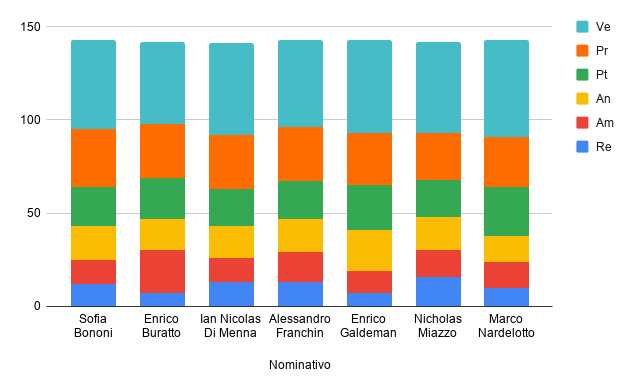
\includegraphics[width=12cm]{img/ore-totale.png}
      \caption{Istogramma della distribuzione totale delle ore}
      \label{fig:ore-totali}
    \end{figure}

    \paragraph{Totale prospetto economico}
    La suddivisione delle ore per ruolo nel totale delle ore investi e rendicontate è la seguente:
    \begin{table}[H]
      \centering
      \begin{tabular}{lcc}
        Ruolo           & Ore previste & Costo                \\
        Responsabile    & 78           & € 2.340,00           \\
        Amministratore  & 105          & € 2.100,00           \\
        Analista        & 124          & € 3.100,00           \\
        Progettista     & 153          & € 3.366,00           \\
        Programmatore   & 214          & € 3.210,00           \\
        Verificatore    & 323          & € 4.845,00           \\
        \textbf{Totale} & \textbf{997} & \textbf{€ 18.961,00}
      \end{tabular}
      \caption{Prospetto economico totale delle ore investite e rendicontate}
    \end{table}

    Per facilitare la lettura della suddivisione oraria per ruolo, i dati vengono rappresentati graficamente mediante il seguente areogramma:
    \begin{figure}[H]
      \centering
      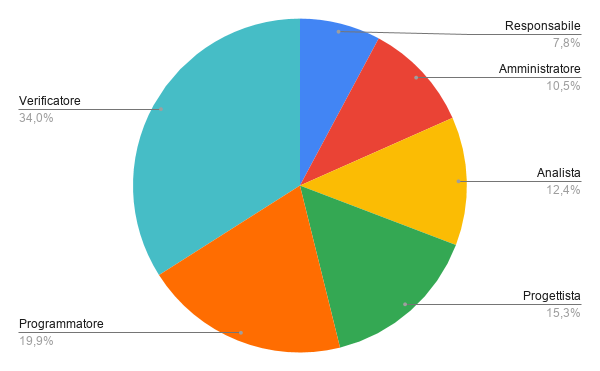
\includegraphics[width=12cm]{img/ruoli-totale.png}
      \caption{Areogramma della suddivisione dei ruoli nel totale delle ore investite e rendicontate}
      \label{fig:ore-totali}
    \end{figure}

    %%%%%%%%%%%%%%%%%%%%%%%%%%%%%%%%%%%%%%%%%%%%%%%%%%%%%%%%%%%%%%%%%%%%%%%%%%%%%%%%%%%%%%%%%%%%%%%%%%%%%%%%%%%%%%%%%%%%%%%%%%%

    \subsubsection{Ore rendicontate}

    \paragraph{Suddivisione del lavoro}
    Di seguito viene il totale delle ore rendicontate a carico del committente:
    \begin{table}[H]
      \begin{tabular}{lccccccc}
        Nominativo                & Re          & Am          & An          & Pt           & Pr           & Ve           & Ore totali   \\
        Sofia Bonomi              & 9           & 5           & 4           & 21           & 33           & 33           & 105          \\
        Enrico Buratto            & 7           & 9           & 6           & 22           & 31           & 30           & 105          \\
        Ian Nicolas Di Menna      & 4           & 7           & 8           & 20           & 31           & 35           & 105          \\
        Alessandro Franchin       & 4           & 13          & 5           & 20           & 31           & 32           & 105          \\
        Enrico Galdeman           & 7           & 5           & 4           & 24           & 32           & 33           & 105          \\
        Nicholas Miazzo           & 6           & 14          & 4           & 20           & 27           & 34           & 105          \\
        Marco Nardelotto          & 7           & 5           & 5           & 26           & 29           & 33           & 105          \\
        \textbf{Ore totali ruolo} & \textbf{44} & \textbf{58} & \textbf{36} & \textbf{153} & \textbf{214} & \textbf{230} & \textbf{735}
      \end{tabular}
      \caption{Distribuzione oraria nel totale delle ore rendicontate}
      \end{table}
  
      Per facilitare la lettura della distribuzione oraria, i dati vengono rappresentati graficamente il seguente istogramma:
      \begin{figure}[H]
        \centering
        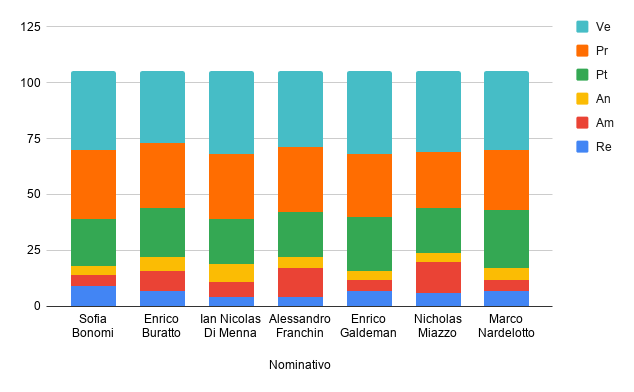
\includegraphics[width=12cm]{img/ore-rendicontate.png}
        \caption{Istogramma della distribuzione totale delle ore}
        \label{fig:ore-rendicontate}
      \end{figure}
  
      \paragraph{Totale prospetto economico}
      La suddivisione delle ore per ruolo nel totale delle ore rendicontate è la seguente:
      \begin{table}[H]
        \centering
        \begin{tabular}{lcc}
          Ruolo           & Ore previste & Costo                \\
          Responsabile    & 44           & € 1.320,00           \\
          Amministratore  & 58           & € 1.160,00           \\
          Analista        & 36           & € 900,00             \\
          Progettista     & 153          & € 3.366,00           \\
          Programmatore   & 214          & € 3.210,00           \\
          Verificatore    & 230          & € 3.450,00           \\
          \textbf{Totale} & \textbf{735} & \textbf{€ 13.406,00}
        \end{tabular}
        \caption{Prospetto economico totale delle ore rendicontate}
      \end{table}
  
      Per facilitare la lettura della suddivisione oraria per ruolo, i dati vengono rappresentati graficamente mediante il seguente areogramma:
      \begin{figure}[H]
        \centering
        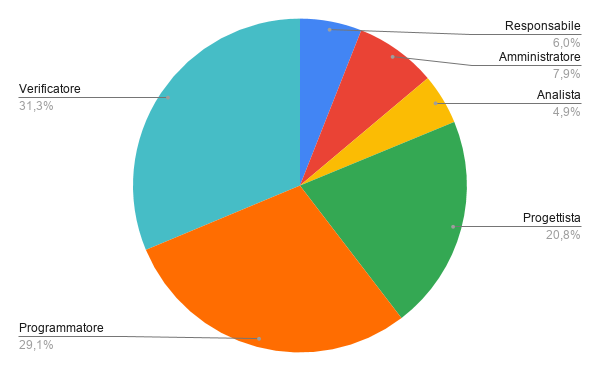
\includegraphics[width=12cm]{img/ruoli-rendicontati.png}
        \caption{Areogramma della suddivisione dei ruoli nel totale delle ore rendicontate}
        \label{fig:ore-rendicontate}
      \end{figure}
  
  \end{document}
